\documentclass[crop,tikz]{standalone}% 'crop' is the default for v1.0, before it was 'preview'
\usepackage{tikz,calc,pgfplots}
\usepackage{tikz-3dplot}
\usetikzlibrary{calc}
\begin{document}

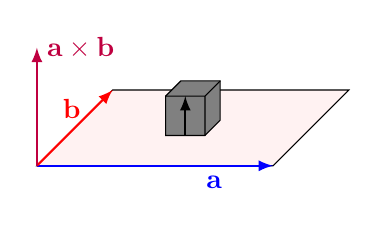
\begin{tikzpicture}[
sensor/.style={black,fill opacity=1,,fill=gray,line cap =round,}]


\draw[fill=white!95!red] (0,0,0) -- (3,0,0)  -- (3,0,-2.5) -- (0,0,-2.5) -- cycle;
\draw[blue,thick,-latex] (0,0,0) -- (3,0,0) node [below,pos=0.75] {$\mathbf{a}$};
\draw[red,thick,-latex] (0,0,0) -- (0,0,-2.5) node [left,pos=0.75,xshift=-1] {$\mathbf{b}$};
\draw[purple,thick,-latex] (0,0,0) -- (0,1.5,0) node [right] {$\mathbf{a}\times\mathbf{b}$};

	\def \x {1.25}
	\def \y {0}
	\def \z {-1.5}
 	\def \s {0.5}
	\draw[sensor] (\x,\y+\s,\z) -- (\x+\s,\y+\s,\z) -- (\x+\s,\y,\z) -- (\x+\s,\y,\z+\s) -- (\x,\y,\z+\s) -- (\x,\y+\s,\z+\s) -- cycle;
	\draw[black,line cap=round] (\x+\s,\y+\s,\z+\s) -- (\x,\y+\s,\z+\s) (\x+\s,\y+\s,\z+\s) -- (\x+\s,\y,\z+\s) (\x+\s,\y+\s,\z+\s) -- (\x+\s,\y+\s,\z);
 
	\draw[black,thick,-latex] (\x+\s/2,\y,\z+\s) -- (\x+\s/2,\y+\s,\z+\s);
\node [] at (0,0) {};
\end{tikzpicture}
\end{document}